\section{Benchmarking and stress testing} \label{chap:Benchmarking}
In this chapter, we present how tests and benchmarks have been conducted, and describe the implementation. 
The goal with the stress tests and benchmarks is threefold: 
\begin{enumerate}
\item It helps us determine the average poll time for clients using the Test Runner under different levels of stress.
\item It helps us decide which configurations to use for the Test Runner system
\item It helps us establish different implementations of the Test Runner component regress in terms of response times.
\end{enumerate}
To conduct the benchmarks, we used BenchmarkDotNet (see chapter \ref{chap:preliminaries}) and defined three components used solely for the benchmarks:
\begin{enumerate}
  \item A client component simulating possible Test Runner client behavior.
  \item A benchmark component responsible for orchestrating benchmarks for different Test Runner versions.
  \item A test component ensuring that the client component can contact the Test Runner before running the benchmarks.
\end{enumerate}


\subsection{Orchestration and Test Runner parameterization}
The benchmark and test components are managed in their own Docker containers, and are connected to a network enabling communication between them and the container hosting the Test Runner. 
Information necessary to establish the connection between Test Runner and other components are defined as environmental constants for the containers, and are passed into the relevant Dockerfiles describing the services.
These constants are then shared among the necessary components' Dockerfile, which then use the information to establish a connection to the Test Runner.
For instance, the environmental constants defining the network location of the Test Runner service is passed as arguments to the Dockerfiles for the tests and the benchmark, as these must both be able to contact the Test Runner service.
These environmental constants also allow easy adjustment of the Test Runner without rebuilding the Docker container.
These include settings such as the size of the queue system and the maximum number of threads the Test Runner can use to process code submissions. 
It is also possible to adjust the time between sweeps and how long each Test Runner result should be stored in memory.
This makes it easy to experiment with different values for the environment variables when performing benchmarks and stress tests.  
The containers are orchestrated such that the benchmarks run only if the test container exits successfully --- that is, all the tests pass successfully. 
Thus, wrongly configured containers do not result in misleading benchmark results.

\subsection{Selecting test parameters}
To achieve a varying degree of complexity for the submission content, several Haskell exercise solutions covering different concepts from course were selected, and Hspec tests based on the description of these problems were developed. 
The code and accompanying tests used in benchmarking and stress testing can be seen in Appendix \ref{chap:TestCode}.
Each file covers a single topic from the course, including recursive type definitions and operations on such types, list comprehension, and filtering of lists. 
One file also contains a syntactical error.
After selecting a representative set of exercises for stress tests and benchmarks a simple operational profile was created, and from this behavioral variables were established: an expected maximum number of clients and different polling times for these clients.
To simulate different platform client behavior, classes representing these were implemented where each class corresponds to a user for a different version of the platform.
These clients implement representations of the necessary behavioral variables, which are annotated using BenchmarkDotNet.
During stress testing, the BenchmarkDotNet framework creates all possible combinations of the implemented behavioral variables.
The underlying implementation of the client classes use an HTTP client.
To evaluate stress test and benchmark results of the developed Test Runner component, we first establish a baseline to compare against.
To establish such baseline, we have stress tested and benchmarked a version of the Test Runner based on the Rocket crate.
This version represents our initial MVP, meaning it runs synchronously and processes only one code submission at a time.
The benchmark for the baseline utilizes the same parameterization as the benchmark for the queue system.
However, it does not poll for the Test Runner result since this version does not respond with a token; instead, it directly responds to the request with the result of processing the code submission.
We suspect that when the Test Runner experiences stress, the synchronous approach will experience a form of starvation where all responses will take a long time to complete due to the asynchronous processing of the request, as each request will have to compete for CPU usage with all other requests.

\subsubsection{Ensuring simultaneous client submissions}
When performing stress tests, one must ensure that the behavior stresses the system in a manner that is realistic but still at the limit of what is probable.
In the case of the Test Runner component, this means exposing it to numerous simultaneous requests. 
To ensure that all submissions to the component happens mostly simultaneously, a method creating a number of actions and invoking them as tasks in close succession (see \ref{lst:TaskBuilder}, line 38 --- 54). 
The method takes an inputted action and wraps it in several other actions, which are then invoked in a loop. 

\begin{lstlisting}[language=CSharp, escapechar=~, caption={C\# code showing the \texttt{BuildClientTaskList} method, which is used to build a number of actions which are executed simultaneously in a Task}, label={lst:TaskBuilder}]
public static class TaskBuilder
{
  public static IEnumerable<Task> BuildClientTaskList<T>
  (int count, Action<T> action)
   where T : CodeRunnerClient, new()
  {
    List<Action> clientActions = new(count);
    List<Task> tasks = new(count);
    
    for (int i = 0; i < count; i++)
    {
        T client = new();
        clientActions.Add(() => action.Invoke(client));
    }

    foreach (Action clientAction in clientActions)
    {
        tasks.Add(Task.Run(clientAction));
    }
    return tasks;
  }
}
\end{lstlisting}

\subsubsection{Baseline benchmark implementation}
The baseline benchmarks seen in listing \ref{lst:baselineBench} is executed multiple times for all combinations of code submissions and number of clients.
The benchmark itself measures the time it takes for all clients to post the code submission and receive an HTTP response with status code 200.
If just one of the submissions cannot be processed, an exception is thrown and the benchmark stops.
It utilizes the \texttt{BuildClientTaskList} method seen in listing \ref{lst:baselineBench}.
\begin{lstlisting}[language=CSharp, escapechar=~, caption={C\# code showing the benchmark implementation for the synchronous baseline}, label={lst:baselineBench}]
// Attributes excluded
public class RocketBenchmarks
{
    [Params(10, 20, 50, 100)] 
    public int NumberOfRequests { get; set; }
    [ParamsSource(nameof(CodeSubmissions))]
    public CodeSubmission CodeSubmission { get; set; }
    public static IEnumerable<CodeSubmission> 
      CodeSubmissions => CodeLoader.Load();

    [Benchmark]
    public void PostAndWaitForResponseReceived()
    {
      IEnumerable<Task> clientActions = TaskBuilder
      .BuildClientTaskList<CodeRunnerClient>
      (
        NumberOfRequests,
        client => client.Post(CodeSubmission)
        .Result.EnsureSuccessStatusCode()
      );
        
      Task.WhenAll(clientActions).Wait();
    }
}
\end{lstlisting}

\subsubsection{Queue system benchmark implementation}
The benchmark for the queue system seen in listing \ref{lst:queueSystemBench} is similar to the one in listing \ref{lst:baselineBench}, as it utilizes the method from listing \ref{lst:TaskBuilder} and the parameterization attributes from BenchmarkDotNet.
However, the internal implementation of the client varies, as it needs to poll for the results of the Test Runner after making an initial request.
Therefore, an additional parameter for the benchmark is introduced to examine how often a client should try to poll for a result.
Best case poll time needs to be established to compare it with the baseline component. 
However, due to the nature of online remote communication, it may be necessary to establish which polling times to avoid instead of using the best average response times.
This is because the benchmarks do not consider the physical distance between the client and the server.
\begin{lstlisting}[language=CSharp, escapechar=~, caption={C\# code showing the benchmark implementation for the asynchronous backend}, label={lst:queueSystemBench}]
// Attributes excluded
public class TicketedCodeRunnerBenchmark
{
    [Params(0.5, 1.0, 2.0, 3.0)] 
    public double PollTime { get; set; }
    [Params(10, 20, 50, 100)] 
    public int NumberOfRequests { get; set; }
    [ParamsSource(nameof(CodeSubmissions))] 
    public CodeSubmission CodeSubmission { get; set; }
    public static IEnumerable<CodeSubmission>
     CodeSubmissions => CodeLoader.Load();

    [Benchmark]
    public void PostAndWaitForAllResultsFetched()
    {
      TimeSpan timeBetweenPolls = TimeSpan.FromSeconds(PollTime);
      IEnumerable<Task> clientActions = TaskBuilder
      .BuildClientTaskList<CodeRunnerQueueClient>
      (
        NumberOfConcurrentRequests, 
        client => client.PostAndGetHaskellResultTask(
          CodeSubmission.code,
          CodeSubmission.test,
          timeBetweenPolls)
      );

      Task.WhenAll(clientActions).Wait();
    }
}
\end{lstlisting}

\subsection{Results}
In this section, results of the combined stress tests and benchmarks are presented.
First, the configuration of the stress tests are described.
This is followed by a presentation of the results of the initial Test Runner benchmark results.
These will be used to compare the synchronous baseline with the asynchronous version.

\subsection{Configuration}
The baseline uses a single thread to test the submitted Haskell code.
Thus no parameterization for this version of the Test Runner is necessary.
Benchmarks for the asynchronous Test Runner is configured such that the number of threads and the queue size varies by five. 
All stress tests and benchmarks are run on computers with an AMD EPYC Processor (with IBPB), four CPUs, four logical cores, and four physical cores.
The computers used for the benchmarks run UBUNTU 20.04 as the operating system and have 32 GB of RAM.
All stress tests begin with a warm-up phase where BenchmarkDotNet sends ten consecutive submissions to the Test Runner. 
Then, for each combination of parameters (number of requests, code submission, and polling times) the stress test is timed and repeated 40 times.
This whole process is repeated five times to ensure outliers does not significantly affect the results.

\subsection{Baseline}
\begin{figure}
  \centering
  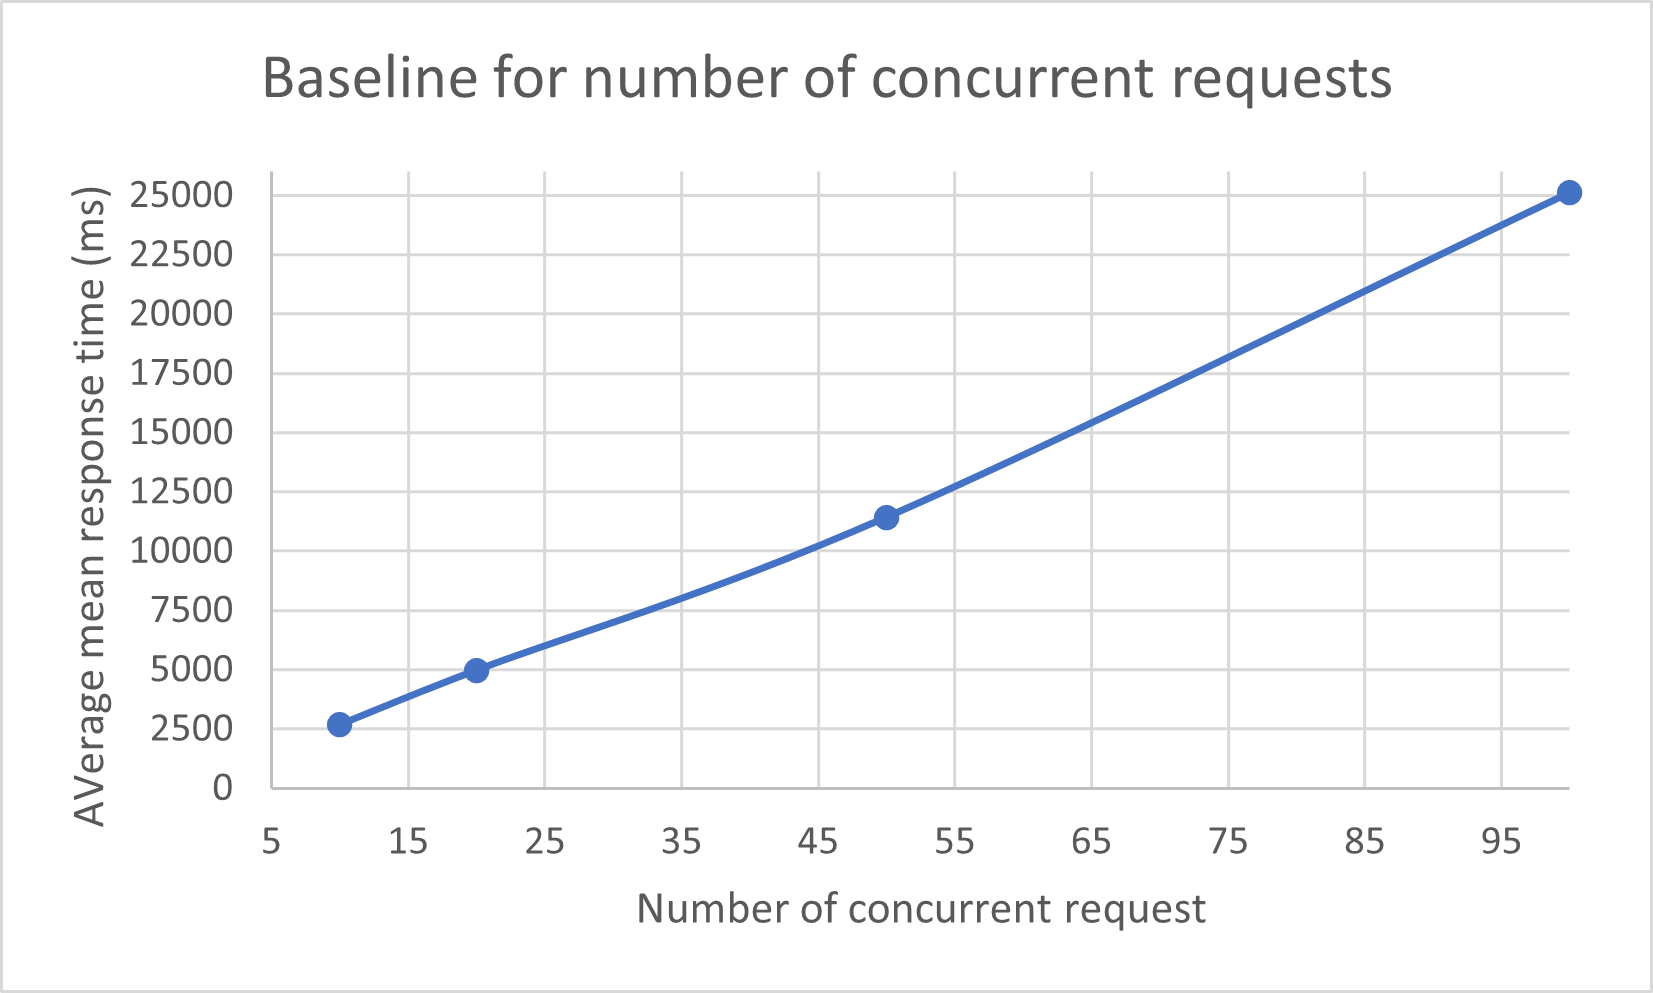
\includegraphics[scale=0.80]{images/baseline.png}
  \caption{The average mean time per request for the baseline Test Runner, disregarding the code submission}
  \label{fig:baseline}
\end{figure}
The synchronous baseline version uses only a single thread to handle all code submissions.
Using this, we can estimate how large of an improvement the asynchronous version is over the synchronous baseline.

Figure \ref{fig:baseline} shows the average mean response time per number of requests for the baseline.
We expect the response time to increase linearly with the number of requests as only one request is handled at a time.
Figure \ref{fig:baseline} shows that this is indeed the case.
The results for the benchmark of the baseline were examined further to see whether some code submissions were slower to process than others (see \ref{chap:AdditionalPlots}). 
We found that only one code submission could be considered a direct outlier, namely the one containing syntactical errors.
This submission was faster to process, likely due to the exercise solution never being executed.



\begin{figure}
  \centering
  \begin{subfigure}[b]{0.45\textwidth}
      \centering
      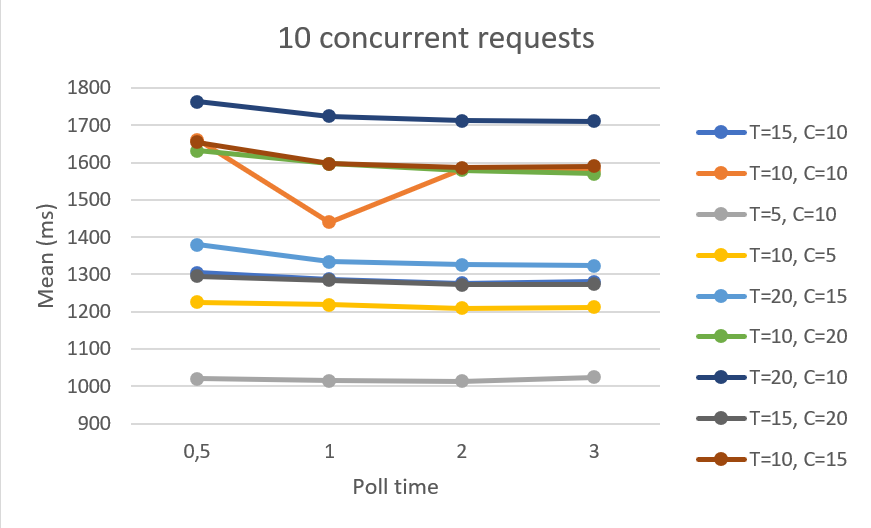
\includegraphics[width=\textwidth]{images/10.png}
      \caption{Mean response time for handling 10 simultaneous client requests for different polling times and Test Runner configurations}
      \label{fig:resultstart}
  \end{subfigure}
  \hfill
  \begin{subfigure}[b]{0.45\textwidth}
    \centering
    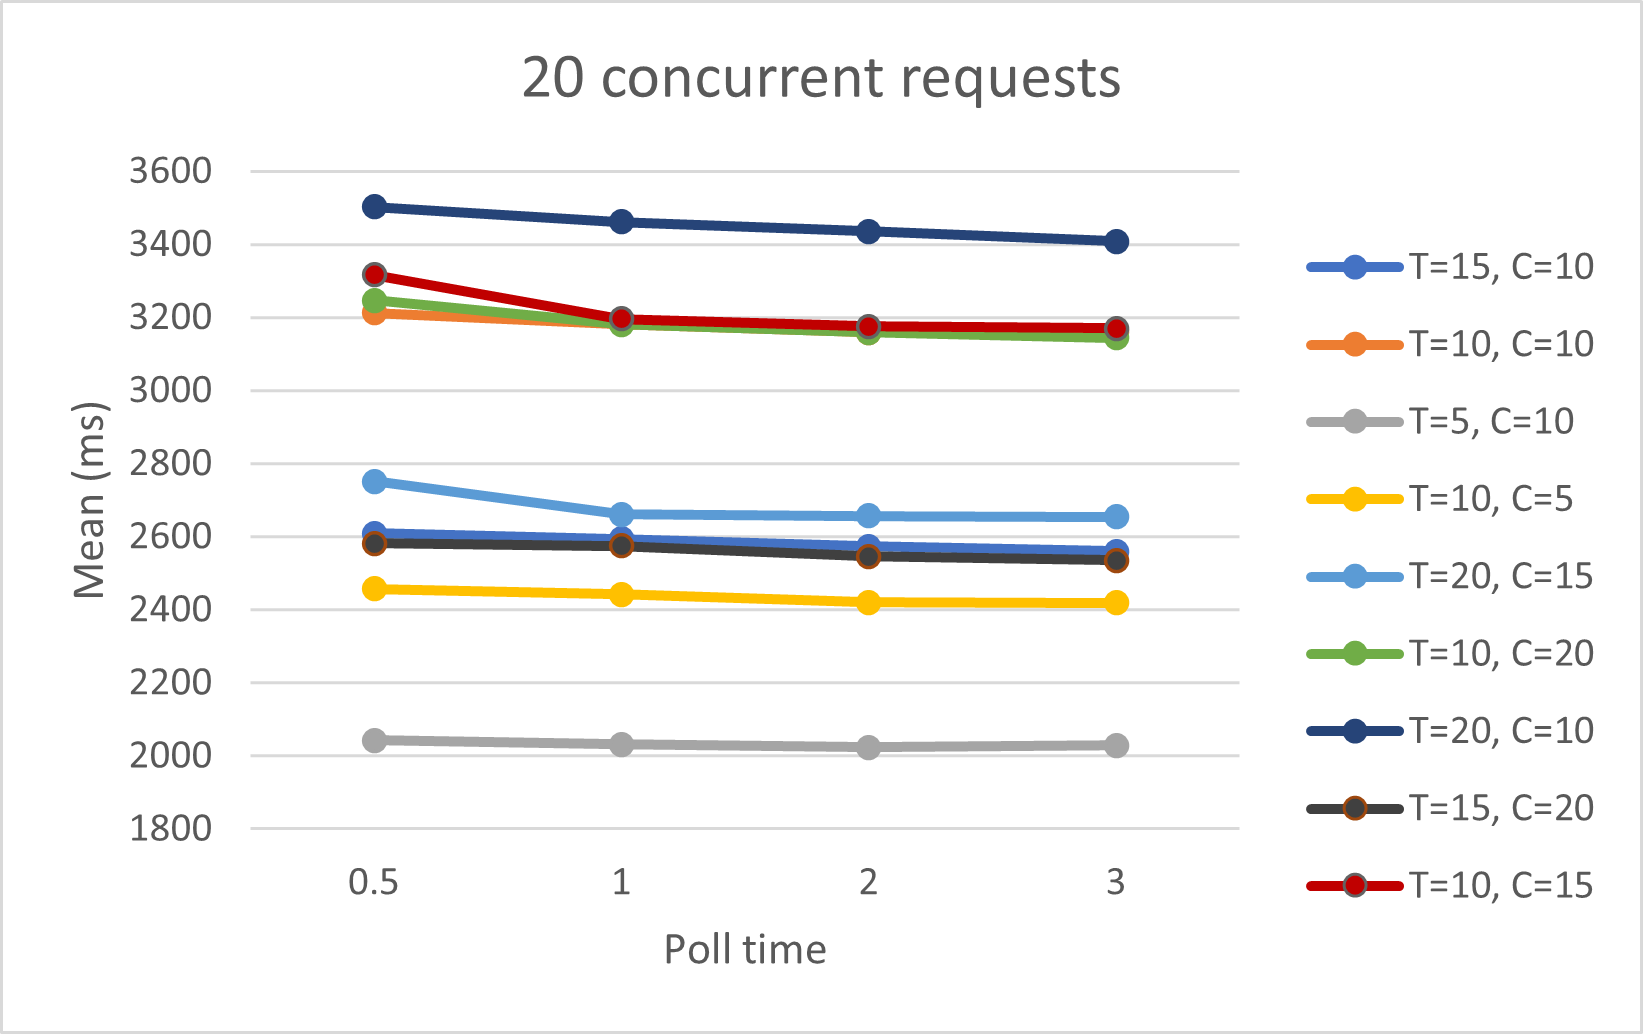
\includegraphics[width=\textwidth]{images/20.png}
    \caption{Mean response time for handling 20 simultaneous client requests for different polling times and Test Runner configurations}
  \end{subfigure}
  \hfill
  \begin{subfigure}[b]{0.45\textwidth}
    \centering
    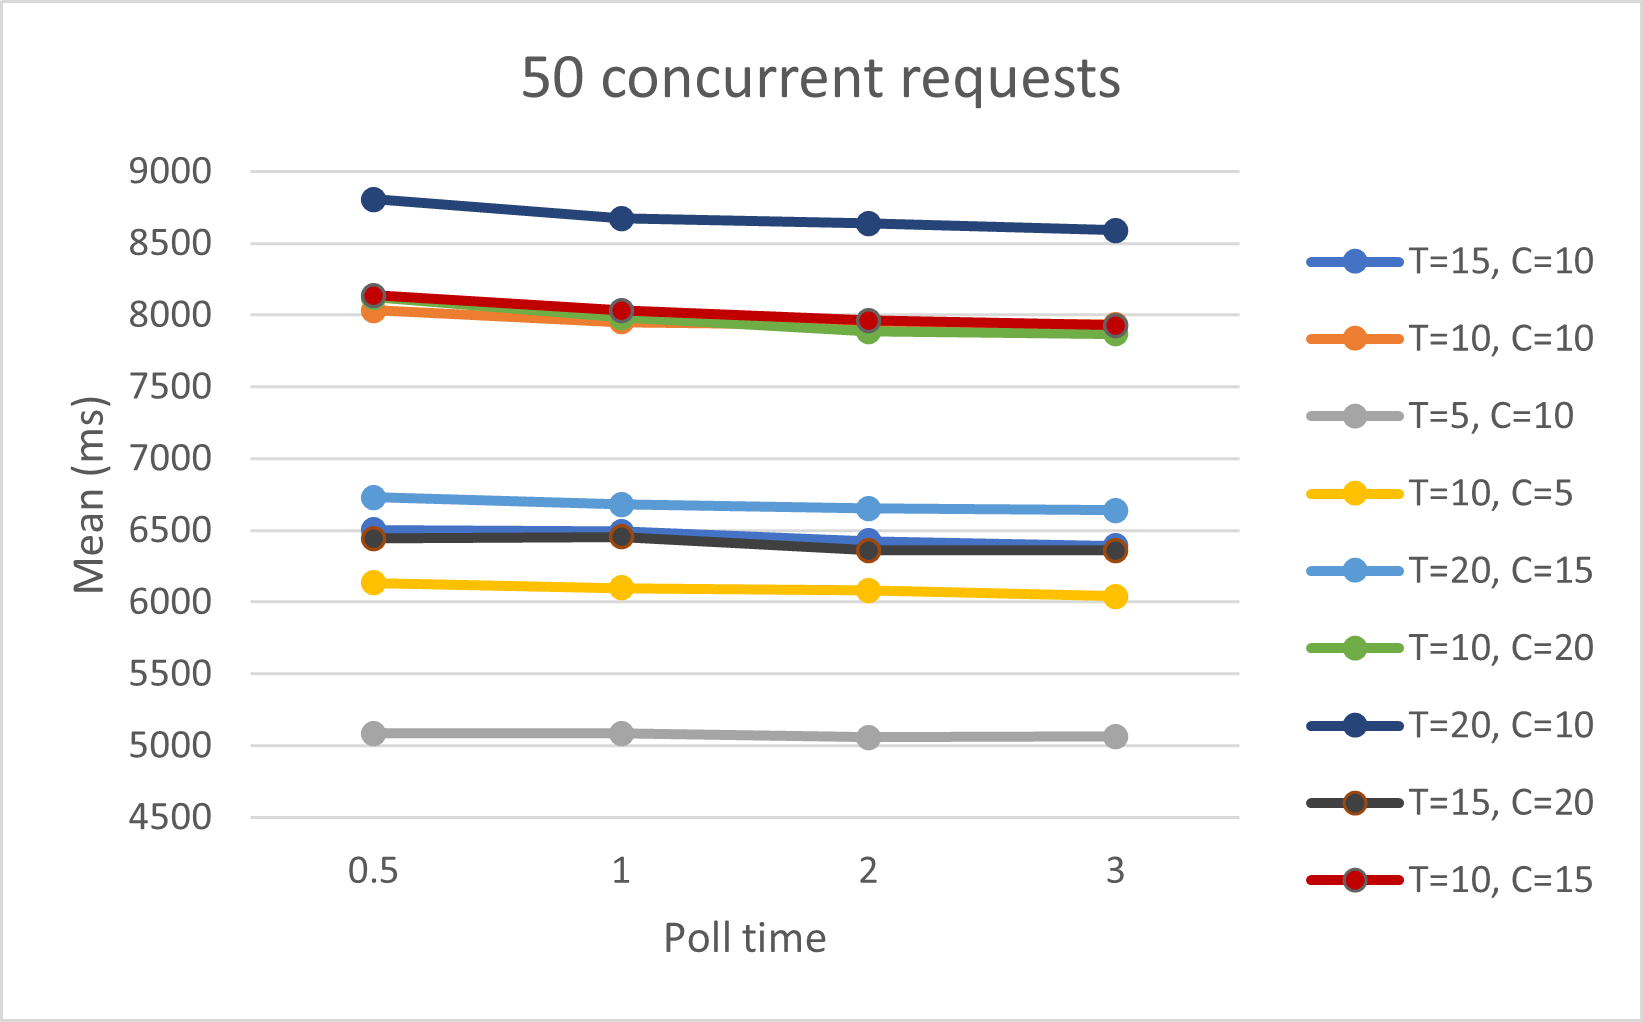
\includegraphics[width=\textwidth]{images/50.png}
    \caption{Mean response time for handling 50 simultaneous client requests for different polling times and Test Runner configurations}
  \end{subfigure}
  \hfill
  \begin{subfigure}[b]{0.45\textwidth}
    \centering
    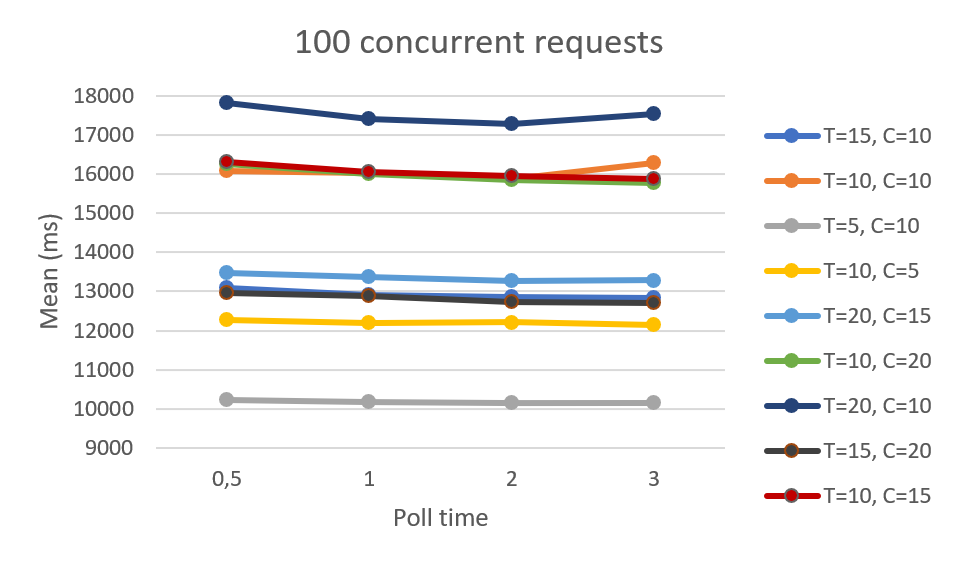
\includegraphics[width=\textwidth]{images/100.png}
    \caption{Mean response time for handling 100 simultaneous client requests for different polling times and Test Runner configurations}
    \label{fig:resultEnd}
  \end{subfigure}
\caption{Mean response time for different asynchronous Test Runner configurations}
\label{fig:configResults}
\end{figure}

Figures \ref{fig:resultstart} --- \ref{fig:resultEnd} shows the mean response time of benchmarking the asynchronous Test Runner with different queue sizes, number of threads, and with clients having varying polling times. 
For each plot, line T denotes the maximum number of threads allowed for testing client submissions, and C denotes the maximum capacity of the channels. 
All the benchmarks shown in figures \ref{fig:resultstart} --- \ref{fig:resultEnd} sweep the result queue every ten seconds, and remove Test Runner results older than 90 seconds. 
Regardless of client polling time, we see that the asynchronous Test Runner with a maximum channel capacity of ten and a maximum of five threads surpasses all other configurations in terms of speed.
Compared to the baseline shown on figure \ref{fig:baseline}, it is vastly superior, requiring only a third of the time to respond to 100 simultaneous requests. 
Since the configuration of the asynchronous Test Runner with five threads and with a channel capacity of ten yields such good results, we examined similar configurations to find a closer estimate to optimal configuration for this particular computer. 
The benchmark results of these configurations can be seen on figure \ref{fig:improvedConfig}.
We see that when the Test Runner is configured correctly, the system can respond to 100 code submissions in under seven seconds.

\begin{figure}
    \centering
    \begin{subfigure}[b]{0.45\textwidth}
        \centering
        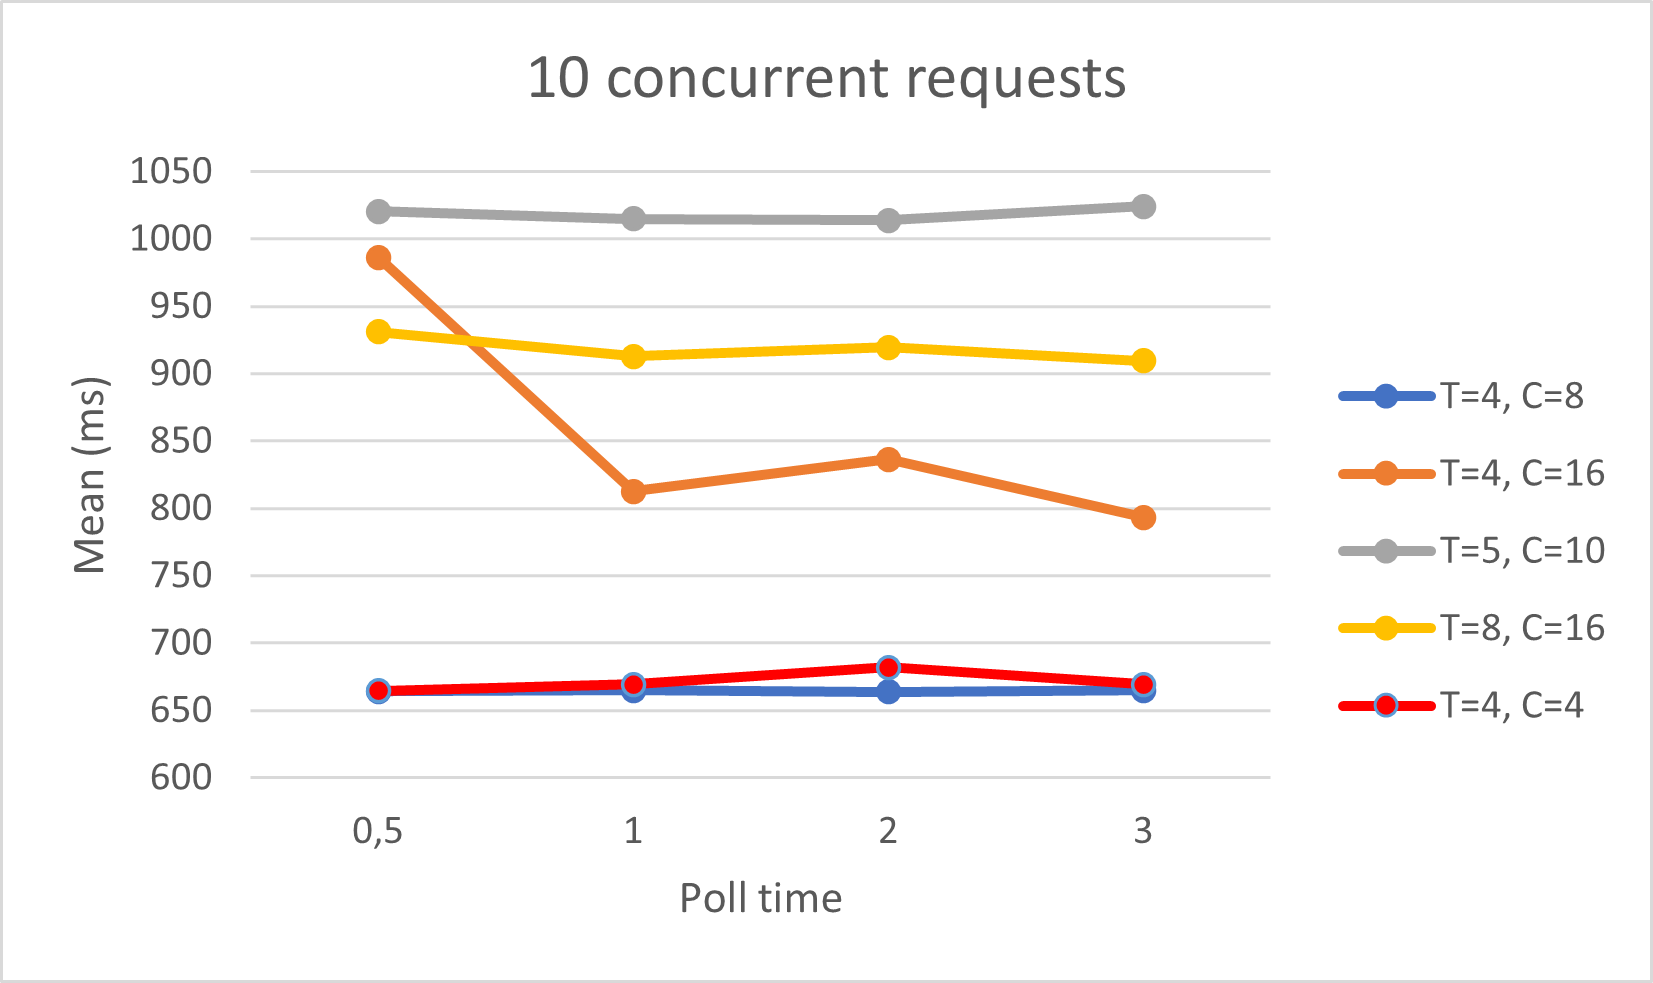
\includegraphics[width=\textwidth]{images/10v3.png}
        \caption{Response times for ten simultaneous requests given improved configurations}
        \label{fig:10v3}
    \end{subfigure}
    \hfill
    \begin{subfigure}[b]{0.45\textwidth}
        \centering
        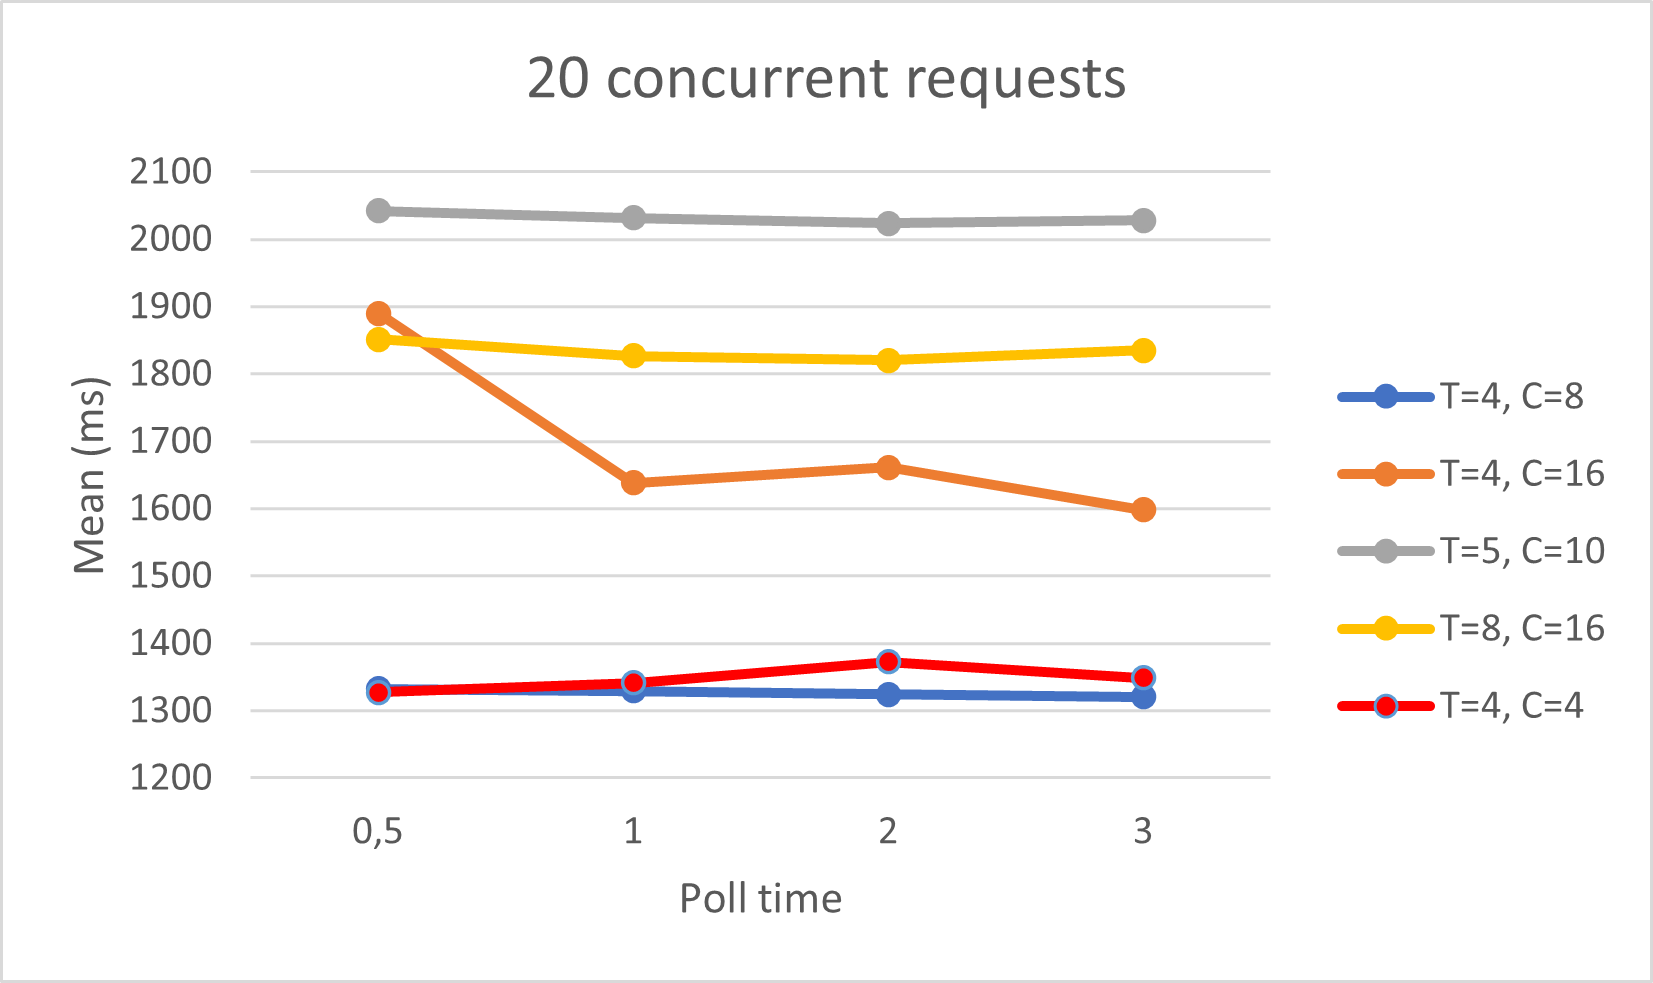
\includegraphics[width=\textwidth]{images/20v3.png}
        \caption{Response times for 20 simultaneous requests given improved configurations}
        \label{fig:20v3}
    \end{subfigure}
    \hfill
    \begin{subfigure}[b]{0.45\textwidth}
        \centering
        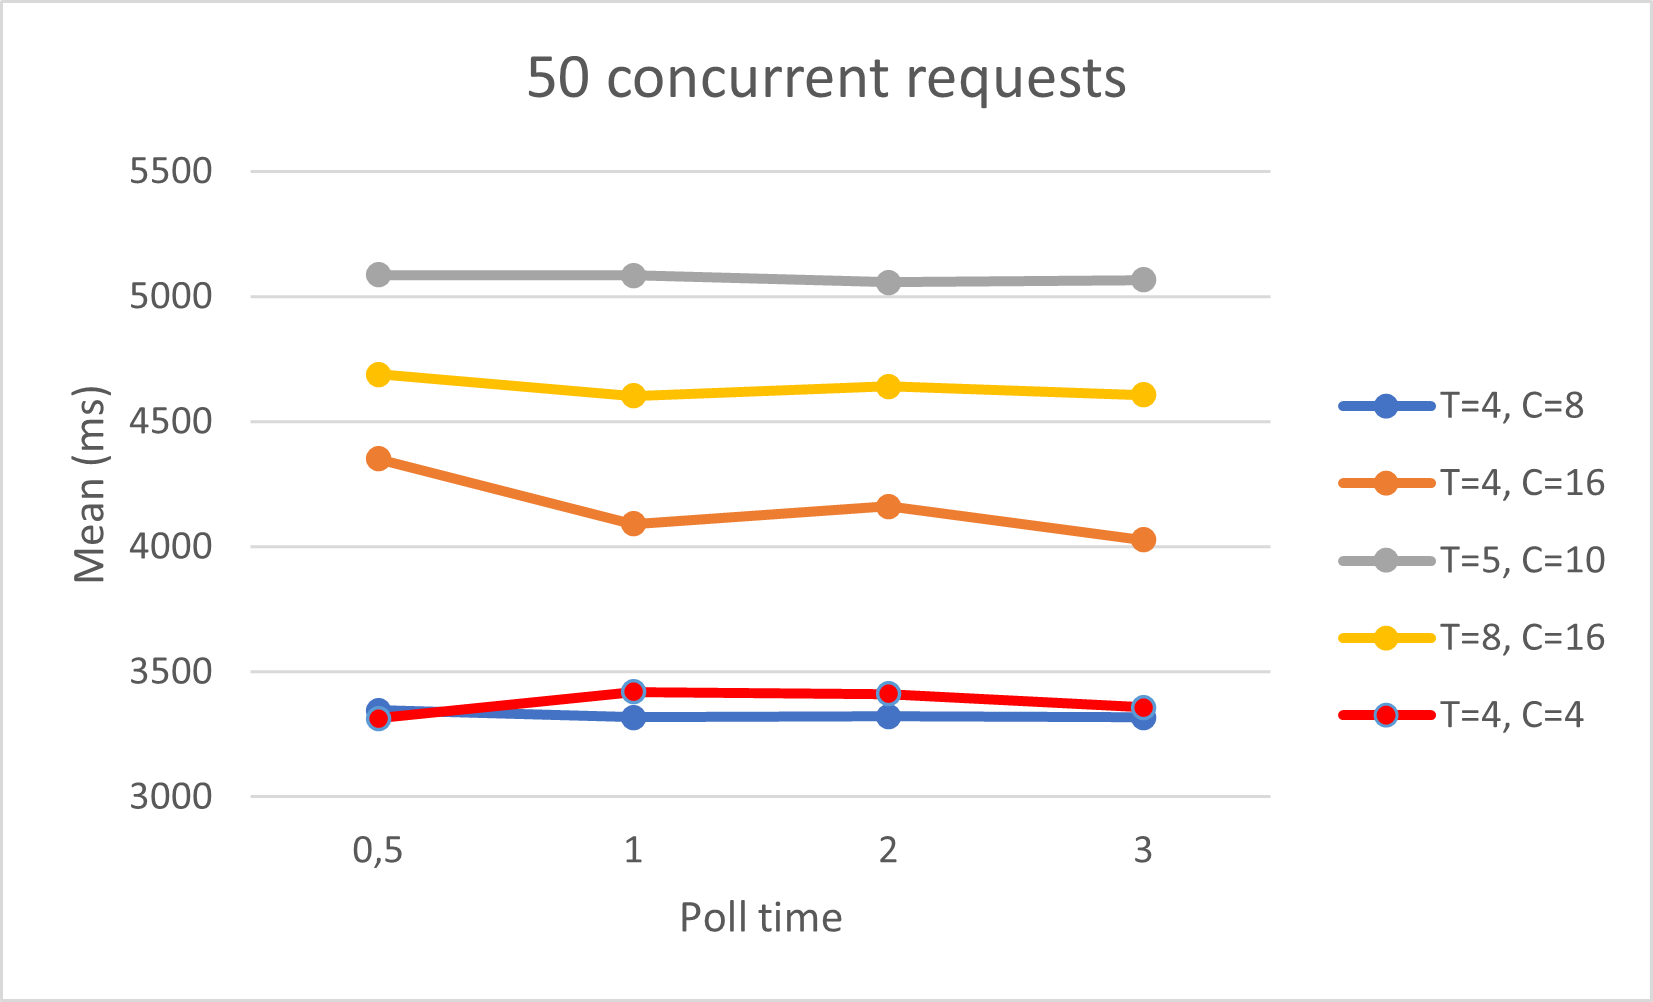
\includegraphics[width=\textwidth]{images/50v3.png}
        \caption{Response times for 50 simultaneous requests given improved configurations}
        \label{fig:50v3}
    \end{subfigure}
    \hfill
    \begin{subfigure}[b]{0.45\textwidth}
      \centering
      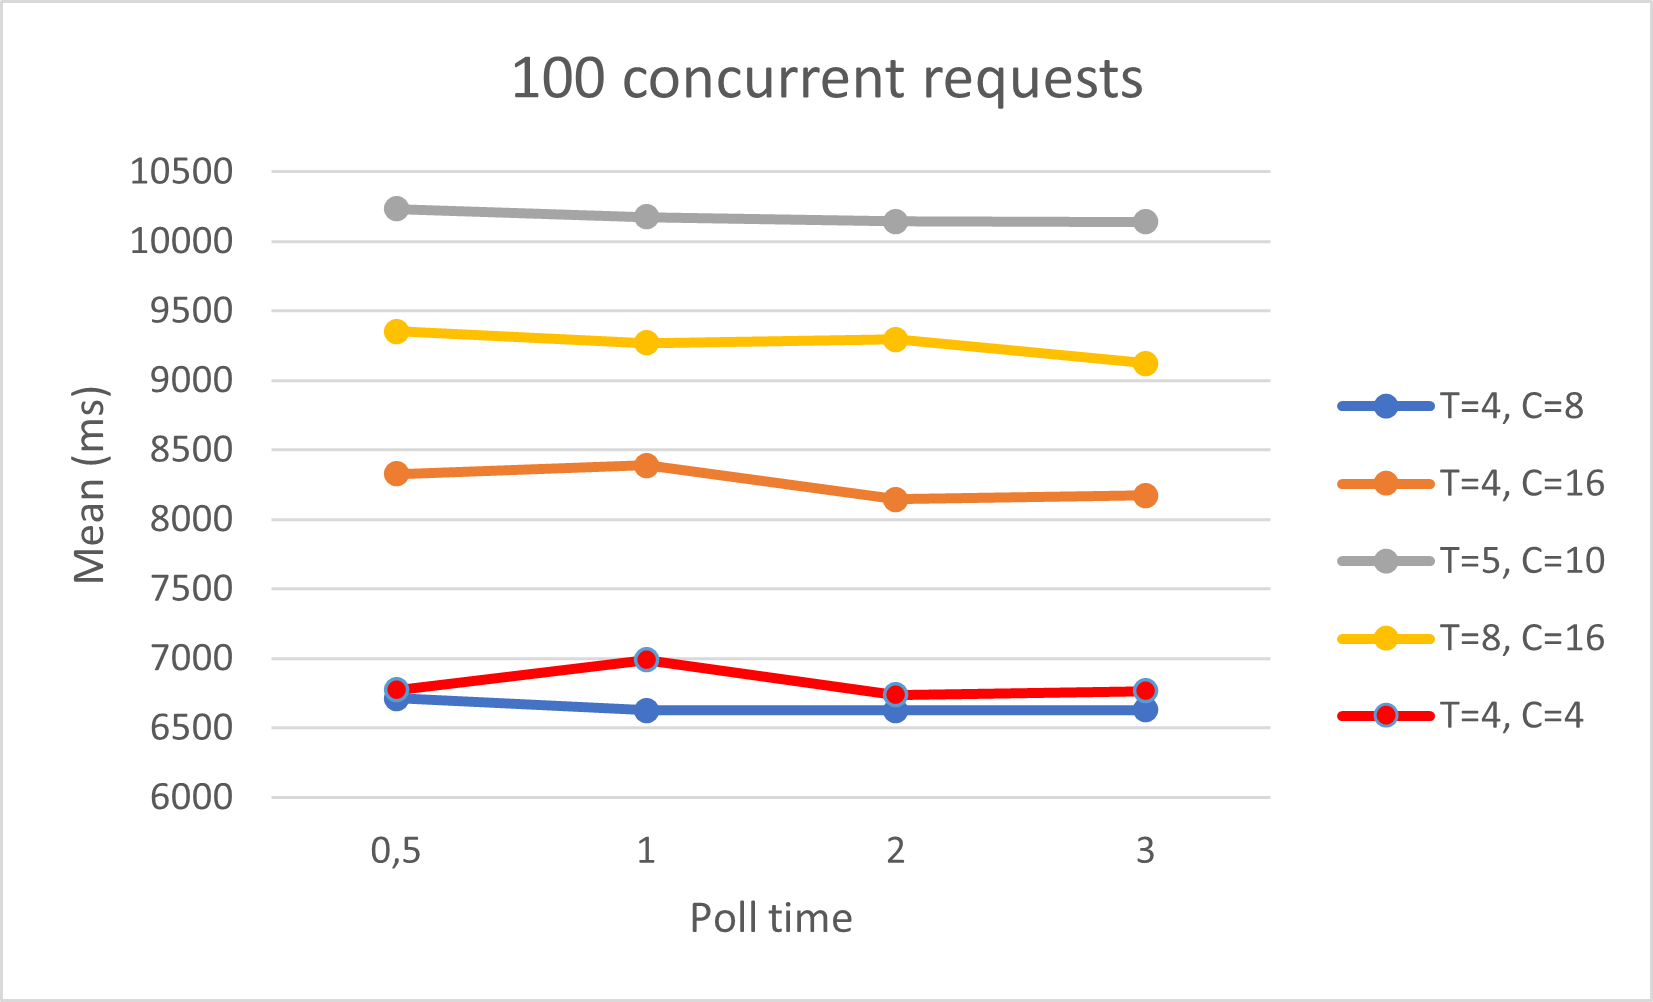
\includegraphics[width=\textwidth]{images/100v3.png}
      \caption{Response times for 100 simultaneous requests given improved configurations}
      \label{fig:100v3}
    \end{subfigure}
  \caption{Response times for Test Runner with configurations similar to the best configuration from figure \ref{fig:configResults}. Note that this configuration is also shown on figures \ref{fig:10v3} --- \ref{fig:100v3}}
  \label{fig:improvedConfig}
\end{figure}